% =====================================================================
% SUPPLEMENTARY NOTE 3 — the limitations, one by one and at length.
%
% AW, 14 November: "Pour your heart out with all the limitations and
% clawing that you can. Here it makes sense because this section is when
% the reader has gone through the paper and understood the good side. Now
% the clawing reads as objective analysis rather than hedging."
%
% The Discussion's limitations paragraph points here ("detailed in
% Supplementary Note 3"). Each item below gives the size, what it touches,
% and the bound on what it can change. Nothing is softened and nothing is
% dramatised; the bound is the point.
%
% CORRECTION RECORDED HERE, 15 November. DISCUSSION_INVENTORY M1 and
% CONTINUITY describe "the split leaks" with 17,873 held-out cells. That
% audit (axw1008/docs/paper/salvage/donor_overlap_58542096) PREDATES commit
% 7ed19bd of 5 October, which resolves the thirty identifiers to fifteen
% people before splitting. Every reported arm was trained after it (the
% p-series from 19 October) and the held-out benchmark counts 70 of 254
% people. What survives is narrower: the WHOLE-CORPUS reads
% (validate_latent.py) key on the raw patient_id, 269 values, so there the
% fifteen people appear twice. Written that way below; flagged to AW.
% =====================================================================

\section{Limitations, at length}
\label{note:limitations}

The Discussion gives the limitations of this work one paragraph. This note
gives each of them the length it needs: what it is, how large it is, which
results it touches, and the bound on how much it can change them. They are
grouped as limits of the data, limits of the estimators and limits of the
claims axis. Where a limitation has a fix that was not built, the fix is
named.

\subsection{Limits of the data}

\paragraph{Fifteen people carry two identifiers.} One study was deposited
twice, under the keys \texttt{garcia\_alonso\_2021\_a} and
\texttt{garcia\_alonso\_2021\_b}, with the same fifteen donors under two sets of donor identifiers and fifteen shared
sample identifiers. The corpus therefore holds 269 donor identifiers for
254 people, and the paper quotes 254 everywhere except where the identifier
is the unit. Three consequences follow, and they differ in whether they
touch a reported number. First, the donor-level split. Identifiers were
reconciled before splitting for every arm reported here: the loader resolves
the thirty identifiers to fifteen people and assigns each person once, so
the held-out set holds 70 of 254 people and no person is on both sides of
the wall. An earlier split, under which seven of the fifteen shared samples
fell on different sides (Table~\ref{stab:split-overlap}) and 17{,}873
held-out cells belonged to a person also present in training, is what
produced the reconciliation; no arm trained under it appears in this paper.
Second, the whole-corpus reads. The validation pass over all 1{,}577{,}728
cells keys on the deposited identifier, so in the whole-corpus cycle
agreement over 142 donors and in the donor-recovery figure over 269 the
fifteen people appear twice, and a neighbour that is the same person under
the other identifier is counted as a cross-donor neighbour. Both deposits
are control endometrium carrying a phase label and no family, severity or
stage label, so the whole-corpus cell-family, severity and stage figures are
untouched and the cycle and donor figures are the two that can be inflated.
The bound is the pair's size, 110{,}336 cells or 7.0\% of the corpus, and
the headline cycle figure, 0.7346, is the held-out one computed on the
reconciled identity. Third, the donor chance rate for donor recovery is
computed over 269 identities, which makes it fractionally lower than over
254 and the enrichment fractionally higher.

\begin{table}[t]
\centering
\caption[The earlier split, sample by sample]{\textbf{The seven of fifteen
shared samples that an earlier donor-level split placed on different sides
of the wall.} Cell counts in parentheses. This split predates every arm
reported here; it is the audit that led to identifiers being reconciled
before splitting.}
\label{stab:split-overlap}
\small
% GENERATED by figures/scripts/supp_figures.py. Do not edit by hand.
\begin{tabular}{@{}lll@{}}
\toprule
sample & in \texttt{garcia\_alonso\_2021\_a} & in \texttt{garcia\_alonso\_2021\_b} \\
\midrule
\texttt{A30} & train (17,000) & test (376) \\
\texttt{E3} & train (3,018) & val (795) \\
\texttt{SAMN15049042} & val (1,958) & train (995) \\
\texttt{SAMN15049043} & val (3,069) & train (990) \\
\texttt{SAMN15049046} & test (2,945) & val (997) \\
\texttt{SAMN15049049} & test (6,737) & train (874) \\
\texttt{SAMN15049051} & train (2,025) & test (996) \\
\bottomrule
\end{tabular}

\end{table}

\paragraph{Label coverage is thin and uneven.} Table~\ref{stab:coverage}
and Supplementary Fig.~\ref{sfig:coverage} give, per study, how many cells
carry each label the paper reads. Cell family comes from two studies,
640{,}606 cells and 118 donors. Menstrual phase comes from three studies
deposited under four keys, 736{,}312 cells. Cycle day, serum progesterone
and epithelial pseudotime come from one study, rASRM stage from one and
surgical grade from another. Six of the eleven studies, 782{,}016 cells and
115 donors, carry no biological annotation at all, which is why the claims
axis rests on transferred labels (Supplementary Note~\ref{note:transfer}).
No cohort records cycle day, stage, grade and hormonal treatment together,
so no within-cohort test of how those variables relate is possible, and
every result that combines them combines cohorts.

\begin{table}[p]
\centering
\caption[Label coverage by study]{\textbf{Cells carrying each label, by
study.} Donor identifiers rather than people, so the two
\texttt{garcia\_alonso} rows share fifteen donors. Six studies carry none
of the eight labels.}
\label{stab:coverage}
\footnotesize\setlength{\tabcolsep}{3pt}
\resizebox{\textwidth}{!}{% GENERATED by figures/scripts/supp_figures.py. Do not edit by hand.
\begin{tabular}{@{}lrrrrrrrrrr@{}}
\toprule
study & cells & donor ids & family & phase & cycle day & progesterone & pseudotime & rASRM stage & grade & cell cycle \\
\midrule
\texttt{duempelmann\_2026} & 466{,}176 & 60 & 465{,}758 & 466{,}176 & 466{,}176 & 466{,}176 & 449{,}850 & -- & 466{,}176 & -- \\
\texttt{fonseca\_2023} & 386{,}560 & 48 & -- & -- & -- & -- & -- & -- & -- & -- \\
\texttt{marecko\_2024} & 174{,}848 & 58 & 174{,}848 & 159{,}800 & -- & -- & -- & 174{,}848 & -- & 174{,}848 \\
\texttt{lin\_2023} & 140{,}032 & 13 & -- & -- & -- & -- & -- & -- & -- & -- \\
\texttt{tan\_2022} & 114{,}944 & 31 & -- & -- & -- & -- & -- & -- & -- & -- \\
\texttt{garcia\_alonso\_2021\_a} & 100{,}096 & 15 & -- & 100{,}096 & -- & -- & -- & -- & -- & -- \\
\texttt{shih\_2022} & 74{,}496 & 11 & -- & -- & -- & -- & -- & -- & -- & -- \\
\texttt{wang\_2022} & 49{,}152 & 4 & -- & -- & -- & -- & -- & -- & -- & -- \\
\texttt{li\_2025} & 45{,}312 & 6 & -- & -- & -- & -- & -- & -- & -- & -- \\
\texttt{ferrero\_2024} & 15{,}872 & 8 & -- & -- & -- & -- & -- & -- & -- & -- \\
\texttt{garcia\_alonso\_2021\_b} & 10{,}240 & 15 & -- & 10{,}240 & -- & -- & -- & -- & -- & -- \\
\midrule
\textbf{all} & 1{,}577{,}728 & 269 & 640{,}606 & 736{,}312 & 466{,}176 & 466{,}176 & 449{,}850 & 174{,}848 & 466{,}176 & 174{,}848 \\
\bottomrule
\end{tabular}
}
\end{table}

\begin{figure}[t]
\centering
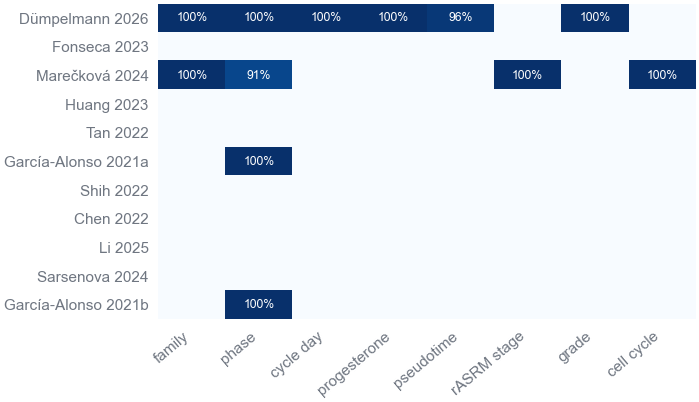
\includegraphics[width=.7\textwidth]{figures/label_coverage_heatmap.png}
\caption[Label coverage, drawn]{\textbf{Share of each study's cells
carrying each label.} Blank is none.}
\label{sfig:coverage}
\end{figure}

\paragraph{The cycle day is one cohort.} The continuous cycle trajectory
rests on \texttt{duempelmann\_2026} alone: 466{,}176 cells from 60 donors,
one day each, days 5 to 30, with 22 of 26 days present and days 20, 24, 25
and 28 absent (Supplementary Fig.~\ref{sfig:cycleday}). No other study
records the day. The closed trajectory is therefore replicated nowhere in
this corpus, and the phase-level results, which draw on three studies, are
the replicated form of the cycle claim.

\begin{figure}[t]
\centering
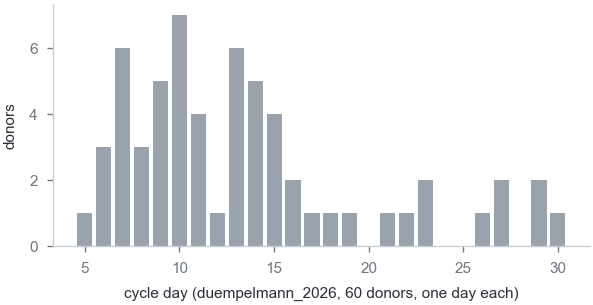
\includegraphics[width=.6\textwidth]{figures/cycle_day_coverage.png}
\caption[Donors per cycle day]{\textbf{Donors per cycle day in the one
cohort that records it.} Red marks the four absent days.}
\label{sfig:cycleday}
\end{figure}

\paragraph{One study is follicular fluid labelled as endometrium.}
\texttt{li\_2025} is a single-cell atlas of pre-ovulatory follicular fluid
collected at oocyte retrieval \citep{li2025iron}. It entered the corpus
labelled as endometrium and the model was conditioned accordingly; tissue is
a decoder covariate, so relabelling the data would mean retraining, and the
label is reported as given. It is 45{,}312 cells, 2.87\% of the corpus, from
six donors, three control and three eutopic, where control marks follicular
fluid from a male-factor infertility patient and eutopic follicular fluid
from an ovarian endometriosis patient. So 2.87\% of the disease axis carries
different semantics from the other 97\%, its cycles are hormonally
stimulated, and it is a fluid aspirate where every other study is a tissue
section. It contributes no cell-family and no phase labels, so the cycle and
cell-type results do not touch it. It is also the one study whose
transferred composition is known to be wrong, because granulosa cells have
no endometrial counterpart (Supplementary Note~\ref{note:transfer}).

\paragraph{Hormonal treatment is inconsistent across cohorts.} Most of
\texttt{tan\_2022}'s thirty-one participants were on hormonal treatment at
sampling; \texttt{duempelmann\_2026} excluded treated participants by design.
Treatment is not a column in any deposit, so it cannot be conditioned on,
and any contrast that spans both cohorts inherits the inconsistency.

\paragraph{Lesion epithelium is confounded with dissociation.} Epithelial
cells are 6.6 times rarer in lesion tissue than in eutopic endometrium,
0.147 against 0.022 of a donor's cells, $P < 0.0001$ over 151 donors
(Supplementary Note~\ref{note:claims}). The study that reports the same
direction attributes it to cell loss during dissociation of fibrous lesion
tissue \citep{sarsenova2024metabolic}. Nothing in this corpus separates
protocol from biology on that contrast, and the result is reported with its
source's caveat rather than as a finding.

\paragraph{One cohort's claims cannot be tested at all.} The deposited
\texttt{shih\_2022} cells are eleven donors, all with disease
\citep{shih2022menstrual}. Its four claims are case against control and
include the largest effect sizes reported anywhere in the corpus, two at
$P < 10^{-16}$. Its controls and its symptomatic-undiagnosed arm are not in
the corpus, so none of the four can be tested here.

\subsection{Limits of the estimators}

\paragraph{The permutation null is unstratified.} The null for every
cross-donor value is built by reassigning the donor-to-label map across all
donors at once and rescoring the fixed neighbour graph. Reassigning across
all eleven studies breaks the link between a label and the study that
carries it, so the null never sees whatever study structure remains in the
latent. If study were fully removed the concern would be void; it is not
fully removed, and the bound on how much it can matter is the reported
arm's own held-out study separation, 0.7613. The correct fix is a
permutation stratified within study, which keeps all 254 people and the
label-to-cohort link together. It is not built.

\paragraph{The null's width is set by donor count.}
Table~\ref{stab:nullwidths} and Supplementary Fig.~\ref{sfig:nullwidths}
give the 95th percentile of the permutation null for every cross-donor
label the reported arm was scored on, with the donor count behind each.
On the held-out split, rASRM stage is carried by 16 donors and its null
reaches 0.42; severity among patients by 18 donors and 0.33. On the whole
corpus the same labels are carried by 57 to 118 donors and their nulls fall
to 0.03 to 0.12. A value that fails its null at 16 donors is undetectable at
that donor count, not absent, and that is how the paper reads it. Which
negatives this bounds: grade, held-out stage, held-out severity among
patients, and the whole-corpus severity among patients, where 0.0744 over 57
donors sits under a null of 0.12.

\begin{table}[t]
\centering
\caption[Null widths against donor count]{\textbf{The permutation null's
95th percentile for every cross-donor label of the reported arm}, with
the donor count that sets it, the observed excess and its $P$. Held out is
the 416{,}256-cell benchmark split; whole corpus is all 1{,}577{,}728 cells.}
\label{stab:nullwidths}
\small
% GENERATED by figures/scripts/supp_figures.py. Do not edit by hand.
\begin{tabular}{@{}llrrrr@{}}
\toprule
scope & label & donors & null$_{95}$ & observed & $P$ \\
\midrule
held out & rASRM stage & 16 & 0.42 & 0.1313 & 0.303 \\
held out & grade & 18 & 0.12 & $-$0.0414 & 0.497 \\
held out & severity, patients only & 18 & 0.33 & $-$0.0968 & 0.781 \\
held out & family & 34 & 0.06 & 0.9820 & 0.005 \\
held out & severity (merged) & 34 & 0.25 & 0.1157 & 0.289 \\
held out & cycle & 36 & 0.18 & 0.7346 & 0.005 \\
whole corpus & severity, patients only & 57 & 0.12 & 0.0744 & 0.129 \\
whole corpus & rASRM stage & 58 & 0.03 & 0.3320 & 0.005 \\
whole corpus & grade & 60 & 0.08 & 0.0263 & 0.408 \\
whole corpus & severity (merged) & 118 & 0.09 & 0.1286 & 0.025 \\
whole corpus (validation) & family & 118 & 0.05 & 0.9807 & 0.005 \\
whole corpus (validation) & cycle & 142 & 0.00 & 0.6796 & 0.005 \\
\bottomrule
\end{tabular}

\end{table}

\begin{figure}[t]
\centering
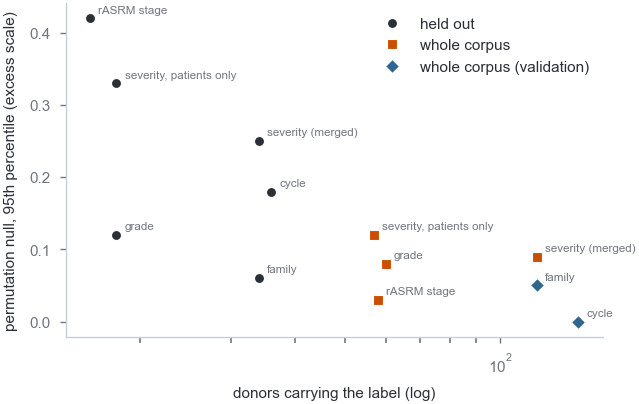
\includegraphics[width=.7\textwidth]{figures/null_width_vs_donors.png}
\caption[Null width falls with donors]{\textbf{Table~\ref{stab:nullwidths}
drawn.} The null narrows as the number of donors carrying a label rises.}
\label{sfig:nullwidths}
\end{figure}

\paragraph{Disease agreement is partly a readout of donor memorisation.}
Across the ten representations in Table~1, cross-donor disease agreement
tracks donor recovery at Spearman $\rho = +0.721$, $P = 0.019$, while
cross-donor cycle agreement does not, at $+0.176$ and $P = 0.627$
(Table~\ref{stab:fieldcorr}, Supplementary Figs.~\ref{sfig:donor-disease}
and~\ref{sfig:donor-cycle}). Disease status is constant within a donor and
the pooled contrast spans studies whose base rates differ, so a
representation that remembers donors is handed part of the label. This is
a caveat on every disease number in the paper including the model's own,
which is the lowest of the ten at 0.3364 and comes from the representation
donors are hardest to recover from. The cycle axis does not have this
property, which is what makes the frontier's biological axis credible.

\begin{table}[t]
\centering
\caption[Correlations across the ten representations]{\textbf{Spearman
rank correlations across the ten representations of Table~1.} Disease
agreement follows donor recovery; the cycle does not.}
\label{stab:fieldcorr}
\small
% GENERATED by figures/scripts/supp_figures.py. Do not edit by hand.
\begin{tabular}{@{}llrr@{}}
\toprule
x & y & Spearman $\rho$ & $P$ \\
\midrule
width & cycle agreement & $-$0.650 & 0.042 \\
donor recovery & disease agreement & 0.721 & 0.019 \\
donor recovery & cycle agreement & 0.176 & 0.627 \\
donor recovery & cell-family agreement & 0.409 & 0.241 \\
\bottomrule
\end{tabular}

\end{table}

\begin{figure}[t]
\centering
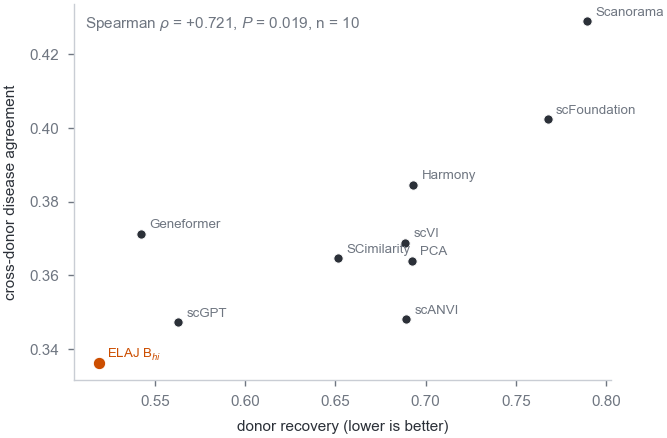
\includegraphics[width=.6\textwidth]{figures/field_donor_vs_disease.png}
\caption[Donor recovery against disease agreement]{\textbf{Donor recovery
against cross-donor disease agreement, ten representations.}}
\label{sfig:donor-disease}
\end{figure}

\begin{figure}[t]
\centering
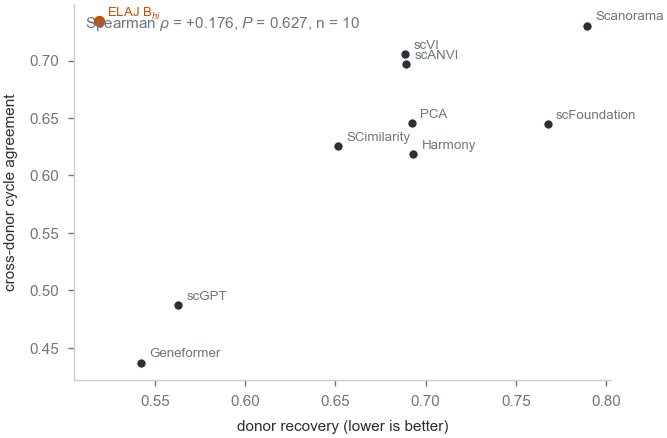
\includegraphics[width=.6\textwidth]{figures/field_donor_vs_cycle.png}
\caption[Donor recovery against cycle agreement]{\textbf{Donor recovery
against cross-donor cycle agreement, ten representations.} The control for
Supplementary Fig.~\ref{sfig:donor-disease}.}
\label{sfig:donor-cycle}
\end{figure}

\paragraph{Representation width is not matched.} \elaj{} has sixteen
dimensions; the comparisons run at their published widths, 16 for principal
components, scVI and scANVI, 50 for Harmony, 100 for Scanorama and 128 to
3{,}072 for the foundation models. The bound on what this can explain runs
the other way: across the ten, width is negatively associated with
cross-donor cycle agreement, $\rho = -0.650$, $P = 0.042$
(Supplementary Fig.~\ref{sfig:width}), and a sixteen-component principal
component decomposition recovers the cycle better than scGPT at 512
dimensions, 0.6457 against 0.4869. Width-matched companions, a
sixteen-component decomposition of each wide embedding scored under the
same protocol, would settle it directly and were not run.

\begin{figure}[t]
\centering
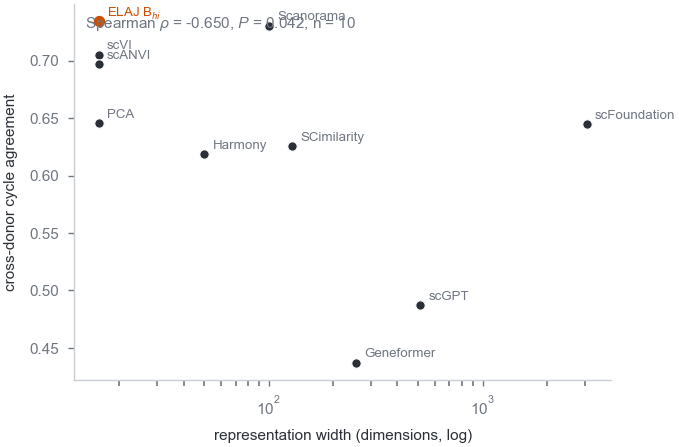
\includegraphics[width=.6\textwidth]{figures/field_width_vs_cycle.png}
\caption[Width against cycle agreement]{\textbf{Representation width
against cross-donor cycle agreement, ten representations}, width on a log
axis.}
\label{sfig:width}
\end{figure}

\paragraph{Every arm is a single run.} The six frontier arms and the five
ablations were each trained once, all at seed 24. No configuration has a
seed replicate, so run-to-run variation is not measured anywhere in the
paper. The registered prediction bands in Supplementary
Notes~\ref{note:frontier} and~\ref{note:ablations} are the only calibration
of how far an arm can land from expectation, and they are not a seed study.
A second seed of \elaj\,B\textsubscript{hi} is the experiment that would
bound it.

\paragraph{The technical controls are best-of-sixteen.} The correlations
reported for serum progesterone and epithelial pseudotime take the largest
$|r|$ over the sixteen latent dimensions, and the negative controls scored
under the identical procedure reach 0.3396 for mitochondrial fraction and
0.3366 for genes detected. The margin over the controls, 0.4725 and 0.5801
against 0.34, is real and it is not large, which is why the controls are
quoted in the same sentence.

\subsection{Limits of the claims axis}

\paragraph{Beyond two studies the cell families are predictions.} The
immune disease direction is reported at 118 donors with the studies' own
labels, held-out AUC 0.7084 at $P = 0.015$ over 94 donors, rather than at
207 with transferred labels, where the same procedure gives 0.5960 at
$P = 0.072$ over 162 donors (Supplementary Note~\ref{note:claims}). Immune
stays the strongest compartment and keeps its sign at the larger count, but
the signal does not strengthen with scale. Two explanations are not
separable here: transferred labels add noise, or the nine added studies are
heterogeneous in ways the two annotated ones are not. Neither number should
be quoted alone.

\paragraph{The stromal direction does not generalise.} Inside stromal cells
the held-out disease AUC is 0.5920 at $P = 0.175$, so there is no stromal
direction to push through the decoder. Three of the four gene-level
predictions made by the largest prior atlas concern decidualised stromal
cells and cannot be tested here; the fourth, IGF1 rising in macrophages, can
and does agree, at rank 285 of 15{,}496 towards disease
\citep{mareckova2024heca}.

\paragraph{The vocabulary is coarser than some claims.} The forty-four
pathway groups are cut from Reactome and GO with 250 to 500 genes each
(Supplementary Note~\ref{note:grouping}). Respiratory electron transport
and ATP synthesis is a group of its own; glycolysis, HIF-1 signalling,
glutathione metabolism and AMPK signalling fall inside merged metabolism
groups, and steroid signalling, iron handling and senescence have no group
of their own. A claim made at the resolution of one of those pathways
\citep{sarsenova2024metabolic,li2025iron} cannot be tested on a group that
merges it with others without answering a coarser question than the one
asked, and none was.

\paragraph{The axis stops at four families.} Every composition test runs
on stromal, epithelial, endothelial and immune. The published findings that
converge on vessel-support cells, a 1.6-fold rise in secretory mural cells,
a lesion-specific perivascular population and the largest metabolic
reprogramming in perivascular cells
\citep{duempelmann2026endometrium,tan2022singlecell,sarsenova2024metabolic},
and the less differentiated epithelium reported in lesions
\citep{garciaalonso2021endometrium,tan2022singlecell}, all sit below that
resolution. The corpus holds the donors to test them, 58 with ectopic
tissue, and the labels to do so would have to be transferred at a finer
vocabulary first, which carries the absorption failure described in
Supplementary Note~\ref{note:transfer} into cell types that are rarer and
closer together.
